\documentclass[aps,prl,reprint,superscriptaddress]{revtex4-1}

%--- PACKAGES ---%
% \usepackage[T1]{fontenc}
\usepackage{graphicx}
\usepackage[usenames,dvipsnames]{color}
\usepackage{amsmath,amssymb}
\usepackage{bm}
\usepackage{upgreek}
\usepackage{xspace}
\usepackage{units}
\usepackage{hhline}
\usepackage[vskip=0pt]{quoting}
\usepackage[colorlinks,urlcolor=blue,citecolor=blue,linkcolor=blue]{hyperref}
\graphicspath{{figures/}}
\renewcommand{\arraystretch}{1.5}

%--- TEXT SHORTCUTS ---%
\newcommand{\etal}{et~al.\xspace}
\newcommand{\Rb}{$^{87}$Rb\xspace}
\newcommand{\qmagic}{q_{\text{magic}}\xspace}
\newcommand{\qRmagic}{q_{R,\text{magic}}\xspace}
% \newcommand{\lundblad}{Phys. Rev. Lett. \textbf{118}, 2xxxxx (2017)}
\newcommand{\lundblad}{arXiv:1706.xxxx}

%--- TEXT OPERATORS ---%
\newcommand{\reffig}[1]{\mbox{Fig.~\ref{#1}}}
\newcommand{\refeq}[1]{\mbox{Eq.~(\ref{#1})}}
\newcommand{\refsec}[1]{\mbox{Sec.~(\ref{#1})}}
\newcommand{\note}[1]{\textcolor{ForestGreen}{[\textrm{#1}]}} % Make editorial notes red

%--- MATH OPERATORS ---%
\newcommand{\upd}{\text{d}}
\newcommand{\totalD}[2]{\frac{\upd #1}{\upd #2}}
\newcommand{\partialD}[2]{\frac{\partial #1}{\partial #2}}
\newcommand{\vecop}[1]{\hat{\mathbf{#1}}\xspace}
\newcommand{\expect}[1]{\langle #1 \rangle}
\newcommand{\abs}[1]{\vert #1 \vert \xspace}
\newcommand{\bra}[1]{\langle #1 \vert \xspace}
\newcommand{\ket}[1]{\vert #1 \rangle \xspace}
\newcommand{\braket}[2]{\langle #1 \vert #2 \rangle \xspace}
\newcommand{\vect}[1]{\mathbf{#1}\xspace}
\newcommand{\uvect}[1]{\hat{\mathbf{#1}}\xspace}
\newcommand{\epvec}{\hat{\mathbf{\epsilon}}\xspace}
\newcommand{\jvect}{\mathbf{\tilde{E}}\xspace}
\newcommand{\ham}{\mathcal{H}}

% Underscores in text (from http://tex.stackexchange.com/a/38720)
\catcode`_=12
\begingroup\lccode`~=`_\lowercase{\endgroup\let~\sb}

\begin{document}

\title{Continuously observing the spectrum of a dynamically decoupled spin-1 quantum gas}

\author{R.\,P.~Anderson}
\author{M.\,J.~Kewming }
\author{L.\,D.~Turner}
\affiliation{School of Physics \& Astronomy, Monash University, Victoria 3800, Australia.}

\date{\today}

\begin{abstract}
Quantum systems can be engineered so that their spectra are sensitive to a particular measurand whilst simultaneously impervious to parasitic fluctuations of an environment.
Here we use a minimally perturbative atom-light interface to study the dressed-state energy spectrum of a spin-1 quantum gas continuously and in-situ.
The spins are coupled by a radio-frequency field, whose amplitude sets the frequency band in which oscillating magnetic fields manifest a linear measurand, and we probe the energy spectrum while the system evolves unitarily.
By varying a symmetry-breaking parameter of the Hamiltonian, we find a regime in which two of the dressed states are maximally insensitive (up to fourth-order) in magnetic field fluctuations that are slow compared to the dressed-state splittings.
Moreover, we demonstrate the predictive power of our continuous probe to tune the measurement band and optimize the dynamical decoupling.
This robust system shares the useful hallmarks of quantum metrology platforms; the states are thus termed ``psuedo-clock'' states in a co-published result by Lundblad~\emph{et al.} (Phys. Rev. Lett. \textbf{118}, 2xxxxx (2017)) and are candidates for band-tunable magnetometry and color charge analogues in quantum gases. 
\end{abstract}

\maketitle

\section{Introduction}
\label{sec:introduction}
\begin{itemize}
    \item Minimally insensitive states in other systems, e.g. $\ket{F=1,m=-1} \leftrightarrow \ket{F=2,m=+1}$ at $B=3.23\unit{G}$, and variants thereof (including those insensitive to Rabi frequency variations reported on at Otago in 2016).
    \item Wide utility of these states for clocks, magnetometers (including microwave, e.g. Treutlein), quantum computing, etc.
    \item General message of making the eigenspectrum insensitive to one thing while retaining sensitivity to another; quantum version of common-mode rejection.
    \item Dynamical decoupling in this context.
    \item Motivate continuous measurement, especially in context of measurement bandwidth; it doesn't make sense to measure something in kHz--MHz band using a shot-based ($0.1\unit{Hz}$ or less) readout. Why? Can't react, can't feedback, can't always assume periodicity/repeatability.
    \item From magnetometry perspective, breaking rotational symmetry is bad because you want there to be no anisotropy to the sensitivity. How does this relate to this work?
    \item The parameter $q$ has been tuned using static magnetic fields and with microwave ac Stark shifts of an off-resonantly driven hyperfine transition, to e.g. to traverse the magnetic phase space of a spinor quantum gas, driving quantum quenches, etc.    
\end{itemize}

\begin{figure}
    \centering
    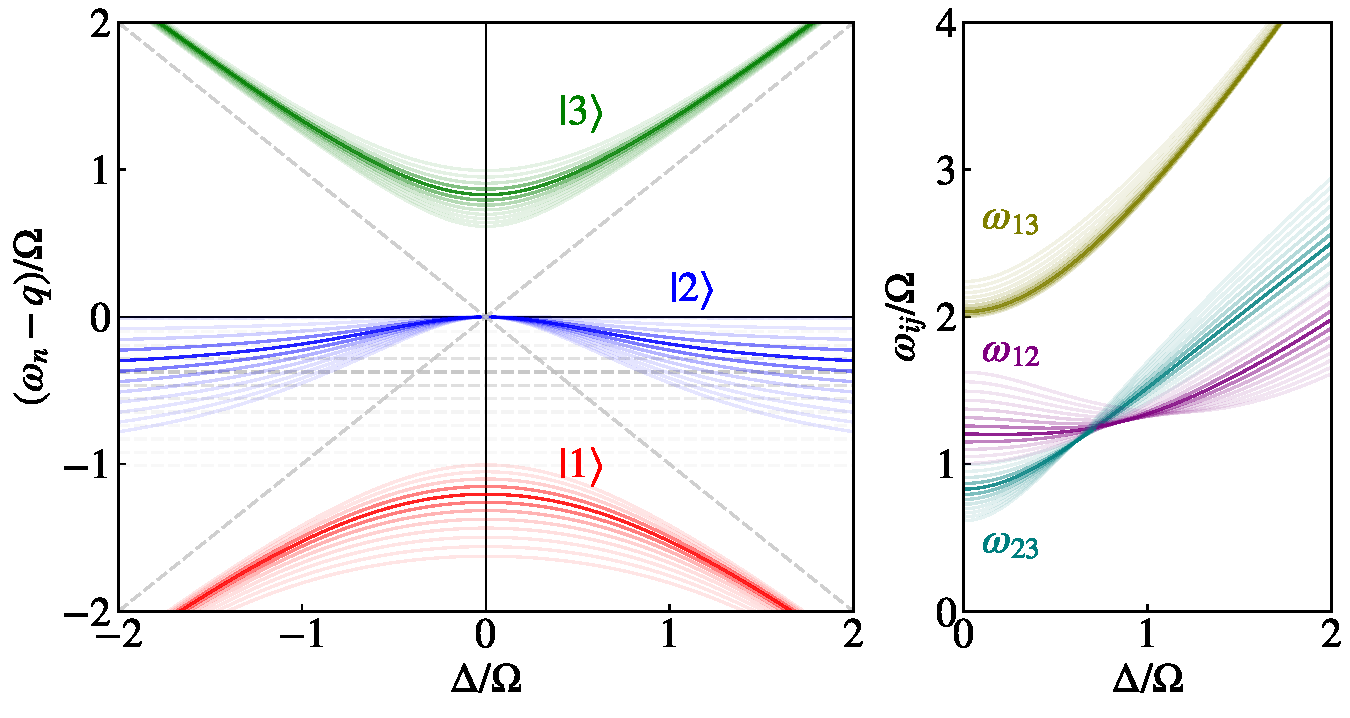
\includegraphics[width=\columnwidth]{figure_1.pdf}
    \caption{
    \label{fig:eigensystem_schematic}
        (Color online)
        Energy spectrum and splittings of a radiofrequency coupled spin-1 for various $q(B)\in[0,\Omega]$.
        The transparency of each curve is proportional to the distance of the quadratic shift $q$ from $\qmagic\approx 0.348\Omega$.
        (Left) Energies $\omega_n$ of dressed states $\ket{n}=\ket{1}$, (red) $\ket{2}$ (blue), and $\ket{3}$ (green) normalized to the rf-coupling strength (Rabi frequency) $\Omega$ as a function of detuning $\Delta(B)=\omega_{\text{rf}}-\omega_L(B)$,
        Dashed lines indicate the energies of uncoupled states ($\Omega=0$) in a frame rotating at $\omega_{\text{rf}}$.
        (Right) Splittings $\omega_{ij}$ of dressed states $\ket{i}$ and $\ket{j}$ as a function of detuning.
        When $q=\qmagic$ (bold curves), energies $\omega_1$ and $\omega_2$ share the same curvature, and their difference $\omega_{12}$ (right, purple) is minimally sensitive to detuning and thus magnetic field variations. 
    }
\end{figure}

\section{Backgound + random}
\label{sec:background}
\begin{itemize}
    \item $\hat{H}_{\text{lab}} = \omega_L \hat{F}_z + q \hat{F}_z^2 + 2\Omega \cos (\omega_{\text{rf}} t) \hat{F}_x \Rightarrow \hat{H}_{\text{RWA}} = -\Delta \hat{F}_z - q \hat{F}_z^2 + \Omega \cos \omega_{\text{rf}} \hat{F}_x$, where $\omega_L(B) \equiv (E_{m=+1} - E_{m=-1})/2 \hbar$ is the Larmor frequency ($\omega_L \propto B$ at low fields but it need not be), $q(B) \equiv (E_{m=+1} + E_{m=-1} - 2 E_{m=0})/2\hbar$ is the quadratic term, as $q\propto B^2$ at low fields (but need not be).
    \item The term $q \hat{F}_z^2$ breaks the $SU(2)$ symmetry of $\hat{H}$, which for $q=0$ is $\hat{H} \propto \vect{B} \cdot \hat{\vect{F}}$ and thus a generator of rotations.
    \item The magnetic field dependence of $\omega_L(B)$ and $q(B)$ can be gleaned from the Breit-Rabi equation, but for our parameters we are justified in using the approximation $f_L = \omega_L/(2\pi) \approx 702379\unit{Hz/G} \times B$ and $q /(2\pi) \approx 71.89\unit{Hz/G^2} \times B^2$.
    \item We vary the magnetic field to affect a change in the detuning of $\Delta \in [0, 2\Omega]$, the domain of \reffig{fig:eigensystem_schematic}(B).
    \item Variations in $B \mapsto B + \Delta B$ of order $B_{\text{rf}} = 2\Omega/\gamma$ affect the detuning linearly, \emph{viz.} $\Delta \mapsto \Delta - \gamma \Delta B$, and do not affect $q$ at all for sufficiently small field strengths.
    \item Indeed, our data corroborate this since we measure $q(B(t))$ across the calibration sweep and find it to be $\sigma(q)/(2\pi) < 5\unit{Hz}$.
    \item Thus the horizontal axis in \reffig{fig:eigensystem_schematic} is a proxy for $\Delta B$, and $\omega_{12}$ at $q=\qmagic$ is has leading-order quartic sensitivity to $\Delta B$.
    \item At high fields ($B\approx 30\unit{G}$) this approximation is no longer valid; $q \approx \qmagic$ varies appreciably across $\Delta B \in [0, B_{\text{rf}}]$ and e.g. $\omega_{12}$ has weak linear dependence on $\Delta B$.
    \item \emph{On varying $\Omega$ or $q$ to change $q_R=q/\Omega$:} At a fixed static magnetic field, $q_R$ can be modified via the Rabi frequency. However, this is not what is represented in \reffig{fig:eigensystem_schematic}, as the normalization of the horizontal and vertical axes would vary for each $q_R$. Importantly, the insensitivity of $\omega_{12}$ to detuning only gets better for increasing $\Omega$ in absolute terms; if the rf amplitude is unlimited, use it. However, doing so also modifies the absolute dressed state splittings on resonance, and thus the bandwidth of the dressed spin-1 as an ac magnetometer. The take home message is then: use as high an rf amplitude as you can afford (or want to tune the ac-band to), and then modify $q_R$ via $q$ to realize the pseudo-clock states.
    \item \textit{Transitions between dressed states:} $\ket{1} \leftrightarrow \ket{2}$ and $\ket{2} \leftrightarrow \ket{3}$ driven by fields oscillating along $y$ or $z$ near frequencies $\omega_D \mp q_D$, respectively. Alternatively, $\ket{1} \leftrightarrow \ket{3}$ driven by fields oscillating along $x$ near frequency $2\omega_D$. This is very different to the fully polarized bare states $\ket{m=\pm 1}$, which are coupled by a single-photon transition as this would conserve neither photon number nor angular momentum. There is no such restriction on the dressed states however as they are neither eigenstates of $\hat{F}_z$ nor photon number. 
\end{itemize}
\textit{Lab frame eigenstates:}
\begin{itemize}
    \item mean splitting $\omega_L$; quadratic shift $q$.
    \item Pairwise coupling between $\ket{m=-1} \leftrightarrow \ket{m=0}$ and $\ket{m=0} \leftrightarrow \ket{m=+1}$ (via $\hat{F}_x$ and/or $\hat{F}_y$, i.e. affected by fields transverse to the static field oscillating near $\omega_L$.
\end{itemize}
\textit{Dressed states on resonance:}
\begin{itemize}
    \item Dressed Larmor frequency:
    \begin{align*}
        \omega_D \equiv (\omega_3 - \omega_2)/2 &= (\omega_{12} + \omega_{23})/2 \\ &= \sqrt{\Omega^2 + q_D^2}\, .
    \end{align*}
    \item Dressed quadratic shift:\\ \[q_D \equiv (\omega_3 + \omega_1 -2\omega_2)/2 = -q/2 \, ,\]
    \item Thus $\Omega = \sqrt{\omega_{12} \omega_{23}}$ and $q_D = (\omega_{23} - \omega_{12})/2$, both of which can be attained from the dressed sideband splittings. This allows (in principle) closed-loop control of $\Omega$ the the atoms. 
    \item Curvature of the dressed-state energies can be evaluated using perturbation theory;
    \[
    \partialD{^2\omega_n}{\Delta^2} = \sum_{k \neq n} \frac{\abs{\bra{k} \hat{F}_z \ket{n}}^2}{\omega_n - \omega_k} \, .
    \]
    \item Thus the curvature of the dressed-state splittings can be found. In particular, the dimensionless curvature of $\omega_{12}$ is (presuming $\abs{\partial q / \partial \Delta} \ll 1$) 
    \begin{align*}
    \partialD{^2(\omega_{12}/\Omega)}{(\Delta/\Omega)^2} &= \Omega \partialD{^2\omega_{12}}{\Delta^2} \\ &= -\frac{3 q_R \sqrt{4 + q_R^2} - q_R^2 - 2}{2 \sqrt{4 + q_R^2}} \, .
    \end{align*}
    This vanishes when $q = \qmagic$, given by
    \[
    \qmagic = \sqrt{(3\sqrt{2} - 4)/2} \approx 0.348 \, .
    \]
    \item Similarly, perturbation theory can be used to show that the third-order derivatives of $\omega_n$ with respect to detuning all vanish when $\abs{\partial q / \partial \Delta} \ll 1$, and thus the leading sensitivity to detuning (and thus $B$) is fourth-order. This validates the choice of our phenomenological even-polynomial model for fitting to $(\Delta B(t), \omega_{12}(t))$ data extracted from Faraday spectrograms.   
\end{itemize}

\bibliography{dressed_faraday}
   
\end{document}
